% files.png: the files a run reads and writes, and what Ansys and Reformat make of them.
% Make it in this folder with, for any scratch folder T:
%   pdflatex -output-directory=T fig_files.tex
%   python3 pdf_to_png.py T/fig_files.pdf ../files.png
\documentclass[11pt,tikz,border=1.5pt]{standalone}
% Shared preamble of all figures. Every fig_*.tex is compiled on its own, see the comment at its top; the fonts are those of the matplotlib
% style xzc_sans (amsmath, amssymb, amsfonts, sfmath), so that line drawings and data plots look the same.
\usepackage{amsmath,amssymb,amsfonts}
\usepackage{sfmath}
\renewcommand{\familydefault}{\sfdefault}
\usepackage{graphicx}
\usetikzlibrary{arrows.meta,calc,positioning,decorations.pathreplacing,backgrounds,shapes.geometric}
% species: Al gray, Mg orange, Zn blue; red marks the vacancy and the jumping atom
\definecolor{cAl}{HTML}{B8BCC2}
\definecolor{cMg}{HTML}{E08A2E}
\definecolor{cZn}{HTML}{3F78B5}
\definecolor{cOne}{HTML}{C8423B}
\definecolor{cTwo}{HTML}{3F78B5}
\definecolor{cThree}{HTML}{3E9B5C}
\definecolor{cFour}{HTML}{E0A21B}
\definecolor{cGray}{HTML}{7E858F}
\definecolor{cDark}{HTML}{2B2B2B}
\newcommand{\panel}[1]{\textbf{(#1)}}
\newcommand{\DM}{D_{\mathrm{MEP}}}
\newcommand{\KI}{K_{\mathrm{I}}}
\newcommand{\KF}{K_{\mathrm{F}}}
\newcommand{\dE}{\Delta E}
\newcommand{\Ea}{\Delta E_{\mathrm{a}}}
\newcommand{\ea}{\Delta e_{\mathrm{a}}}
\newcommand{\Ebind}{E_{\mathrm{bind}}^{\mathrm{site}}}
% a ball with a soft highlight, like the rendered spheres
\makeatletter
\pgfdeclareradialshading[tikz@ball]{softball}{\pgfpoint{-9bp}{9bp}}{%
  color(0bp)=(tikz@ball!22!white); color(6bp)=(tikz@ball!62!white); color(13bp)=(tikz@ball!96!white);
  color(20bp)=(tikz@ball!92!black); color(27bp)=(tikz@ball!74!black); color(50bp)=(tikz@ball!55!black)}
\makeatother
\tikzset{
  every picture/.append style={line cap=round, line join=round},
  every node/.append style={font=\small},
  img/.style={inner sep=0pt, anchor=south west},
  lab/.style={font=\normalsize, inner sep=1pt, anchor=north west},
  above lab/.style={font=\normalsize, inner sep=1pt, anchor=south west},
  capt/.style={align=center, anchor=north},
  atom/.style={circle, ball color=#1, shading=softball, minimum size=12pt, inner sep=0pt},
  atom/.default=cAl,
  vac/.style={circle, draw=cOne, line width=1.1pt, fill=white, minimum size=11.5pt, inner sep=0pt},
  arr/.style={-{Stealth[length=5pt]}, line width=0.8pt},
  dbl/.style={{Stealth[length=4pt]}-{Stealth[length=4pt]}, line width=0.8pt},
  jump/.style={arr, cOne, line width=1.2pt},
  block/.style={-{Triangle[length=8pt, width=13pt]}, line width=5pt, cTwo!38},
  cell axis/.style={-{Triangle[length=6pt, width=5.5pt]}, line width=1.2pt, black},
  dir/.style={fill=white, fill opacity=0.75, text opacity=1, font=\footnotesize, inner sep=1.5pt},
}
\graphicspath{{img/}}
% data plots are included at one scale: \plot{name}{x}{y}{file}
\newcommand{\plotscale}{0.6}
\newcommand{\plot}[4]{\node[img] (#1) at (#2,#3) {\includegraphics[scale=\plotscale]{#4}};}
\newcommand{\plotlabel}[2]{\node[above lab] at ($(#1.north west)+(-0.05,0.02)$) {\panel{#2}};}
% legend of the species, first entry at (#1,#2): Al, Mg, Zn (and the vacancy)
\tikzset{leg/.style={anchor=base west, inner sep=2pt, yshift=-3.2pt}}
\newcommand{\specieslegend}[2]{%
  \foreach \lx/\lc/\lt in {0/cAl/Al, 1.2/cMg/Mg, 2.4/cZn/Zn} {
    \node[atom=\lc, minimum size=10pt] at ({#1+\lx},#2) {}; \node[leg] at ({#1+\lx+0.2},#2) {\lt};}}
\newcommand{\vacancylegend}[2]{\node[vac, minimum size=9.5pt] at (#1,#2) {}; \node[leg] at ({#1+0.2},#2) {vacancy};}

\newcommand{\file}[1]{{\footnotesize\ttfamily\detokenize{#1}}}
\begin{document}
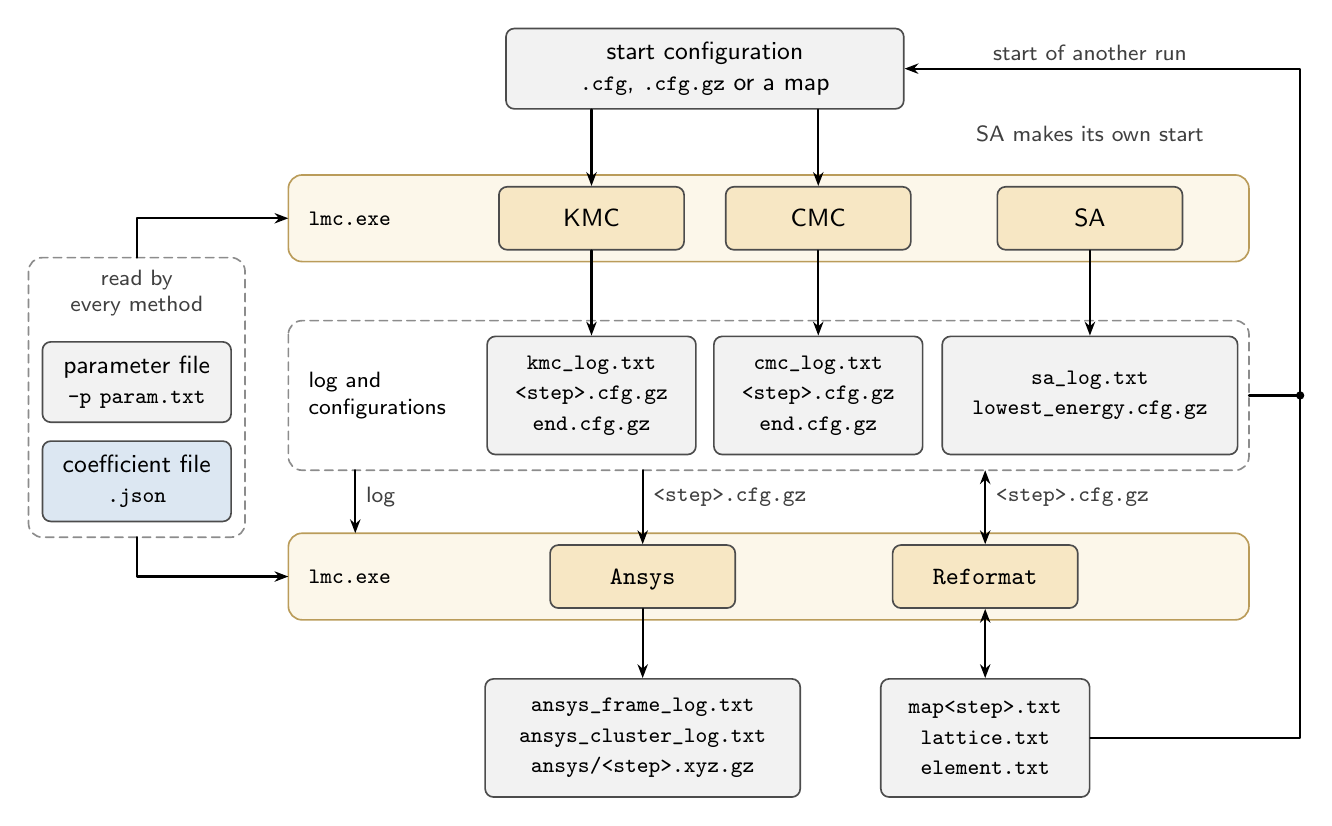
\begin{tikzpicture}[
    box/.style={draw=black!70, rounded corners=3pt, align=center, inner sep=5pt, line width=0.6pt},
    data/.style={box, fill=black!5},
    model/.style={box, fill=cTwo!18},
    algo/.style={box, fill=cFour!26, minimum height=0.8cm, text width=2.0cm, text height=1.55ex, text depth=0.25ex},
    prog/.style={draw=cFour!70!black!70, rounded corners=5pt, fill=cFour!9, line width=0.6pt},
    group/.style={draw=black!45, densely dashed, rounded corners=5pt, line width=0.6pt},
    note/.style={font=\footnotesize, text=black!75, align=center, inner sep=1.5pt},
    row/.style={font=\footnotesize, anchor=west, align=left, inner sep=0pt},
    both/.style={{Stealth[length=5pt]}-{Stealth[length=5pt]}, line width=0.8pt}]
  % ---------------- a run and its start ----------------
  \draw[prog] (3.3,-1.35) rectangle (15.5,-2.45);
  \node[row] at (3.55,-1.90) {\file{lmc.exe}};
  \node[algo] (kmc) at (7.15,-1.90) {KMC};
  \node[algo] (cmc) at (10.03,-1.90) {CMC};
  \node[algo] (sa) at (13.48,-1.90) {SA};
  \node[data, text width=4.7cm] (start) at (8.59,0) {start configuration\\ \file{.cfg}, \file{.cfg.gz} or a map};
  \node[note] at (13.48,-0.83) {SA makes its own start};
  \draw[arr] (kmc.north |- start.south) -- (kmc.north);
  \draw[arr] (cmc.north |- start.south) -- (cmc.north);
  % ---------------- its files ----------------
  \draw[group] (3.3,-3.20) rectangle (15.5,-5.10);
  \node[row] at (3.55,-4.15) {log and\\ configurations};
  \node[data, text width=2.3cm, minimum height=1.5cm] (fkmc) at (7.15,-4.15) {\file{kmc_log.txt}\\ \file{<step>.cfg.gz}\\ \file{end.cfg.gz}};
  \node[data, text width=2.3cm, minimum height=1.5cm] (fcmc) at (10.03,-4.15) {\file{cmc_log.txt}\\ \file{<step>.cfg.gz}\\ \file{end.cfg.gz}};
  \node[data, text width=3.4cm, minimum height=1.5cm] (fsa) at (13.48,-4.15) {\file{sa_log.txt}\\ \file{lowest_energy.cfg.gz}};
  \draw[arr] (kmc) -- (fkmc);
  \draw[arr] (cmc) -- (fcmc);
  \draw[arr] (sa) -- (fsa);
  % ---------------- analysis and conversion ----------------
  \draw[prog] (3.3,-5.90) rectangle (15.5,-7.00);
  \node[row] at (3.55,-6.45) {\file{lmc.exe}};
  \node[algo] (ansys) at (7.80,-6.45) {\ttfamily Ansys};
  \node[algo] (reformat) at (12.15,-6.45) {\ttfamily Reformat};
  \draw[arr] (4.15,-5.10) -- node[note, anchor=west, pos=0.43, xshift=2pt] {log} (4.15,-5.90);
  \draw[arr] (ansys.north |- 0,-5.10) -- node[note, anchor=west, pos=0.36, xshift=2pt] {\file{<step>.cfg.gz}} (ansys);
  \draw[both] (reformat.north |- 0,-5.10) -- node[note, anchor=west, pos=0.36, xshift=2pt] {\file{<step>.cfg.gz}} (reformat);
  \node[data, text width=3.65cm, minimum height=1.5cm] (fansys) at (7.80,-8.50) {\file{ansys_frame_log.txt}\\ \file{ansys_cluster_log.txt}\\ \file{ansys/<step>.xyz.gz}};
  \node[data, text width=2.3cm, minimum height=1.5cm] (fmap) at (12.15,-8.50) {\file{map<step>.txt}\\ \file{lattice.txt}\\ \file{element.txt}};
  \draw[arr] (ansys) -- (fansys);
  \draw[both] (reformat) -- (fmap);
  % ---------------- read by every method ----------------
  \draw[group] (0,-2.40) rectangle (2.75,-5.95);
  \node[note, anchor=north] at (1.375,-2.50) {read by\\ every method};
  \node[data, text width=2.15cm, inner xsep=3.5pt] (param) at (1.375,-3.98) {parameter file\\ \file{-p param.txt}};
  \node[model, text width=2.15cm, inner xsep=3.5pt] (coef) at (1.375,-5.24) {coefficient file\\ \file{.json}};
  \draw[arr] (1.375,-2.40) |- (3.3,-1.90);
  \draw[arr] (1.375,-5.95) |- (3.3,-6.45);
  % ---------------- start of another run ----------------
  \draw[arr] (fmap.east) -- (16.15,-8.50) |- (start.east);
  \draw[line width=0.8pt] (15.5,-4.15) -- (16.15,-4.15);
  \fill (16.15,-4.15) circle (1.5pt);
  \node[note, anchor=south] at (13.48,0.05) {start of another run};
\end{tikzpicture}
\end{document}
